\documentclass{article}
\usepackage[utf8]{inputenc}
\usepackage{graphicx}
\usepackage{amsmath}
\usepackage{amssymb}
\usepackage{subcaption}
\usepackage{float}
\title{Mat4 Aflevering 5}
\author{Roar Nind Steffensen}
\date{March 2016}

\begin{document}

\maketitle

\section*{Problem 5.3}
\begin{figure}[H]
    \centering
    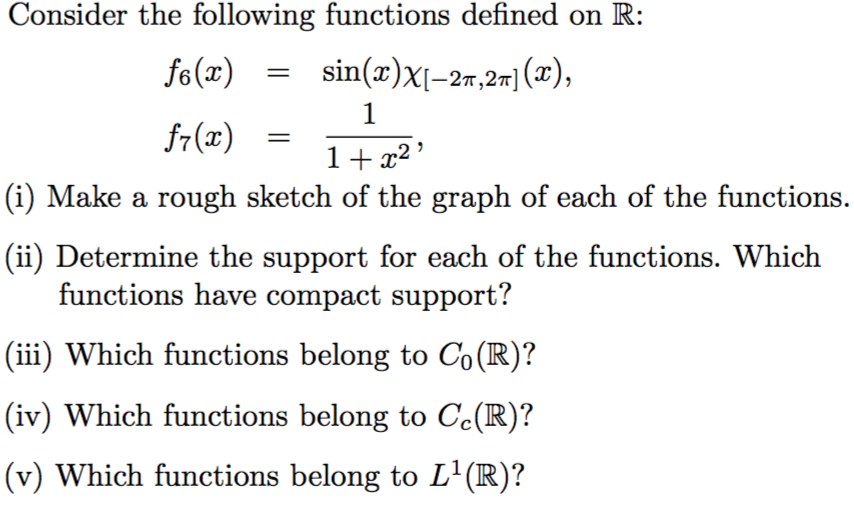
\includegraphics[height=6cm]{fig/prob53}
\end{figure}
\vspace{-0.5cm}
\subsection*{Solution (i)}
First we sketch the functions $f_6(x)$ and $f_7(x)$ \\
\begin{figure}[H]
\centering
    \begin{subfigure}{0.495\textwidth}
    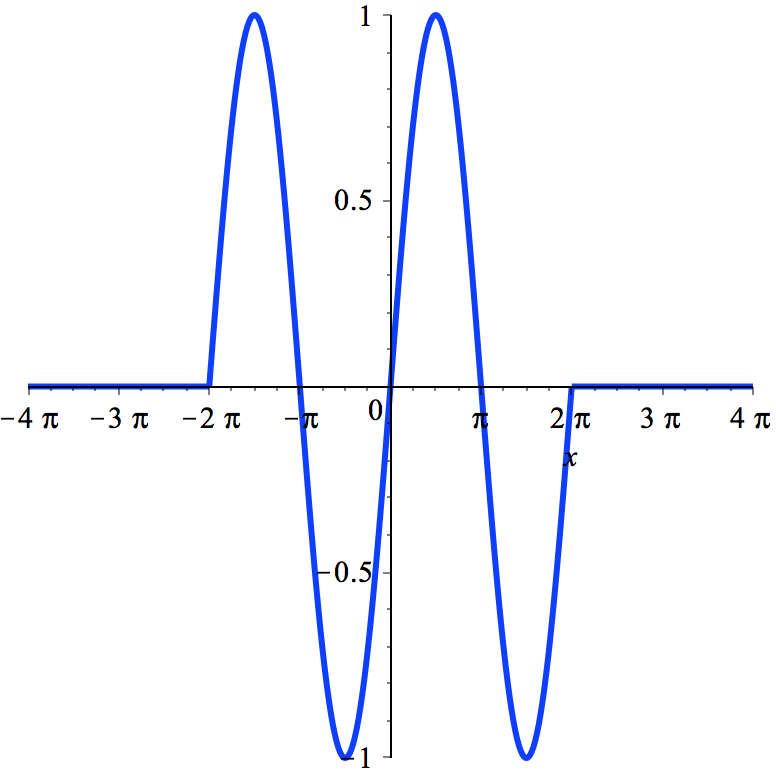
\includegraphics[width=0.9\linewidth, height=4cm]{fig/f6}
    \caption*{$f_6(x)=\text{sin}(x)\chi_{[-2 \pi,2 \pi]}(x)$}
    \end{subfigure}
    \begin{subfigure}{0.495\textwidth}
    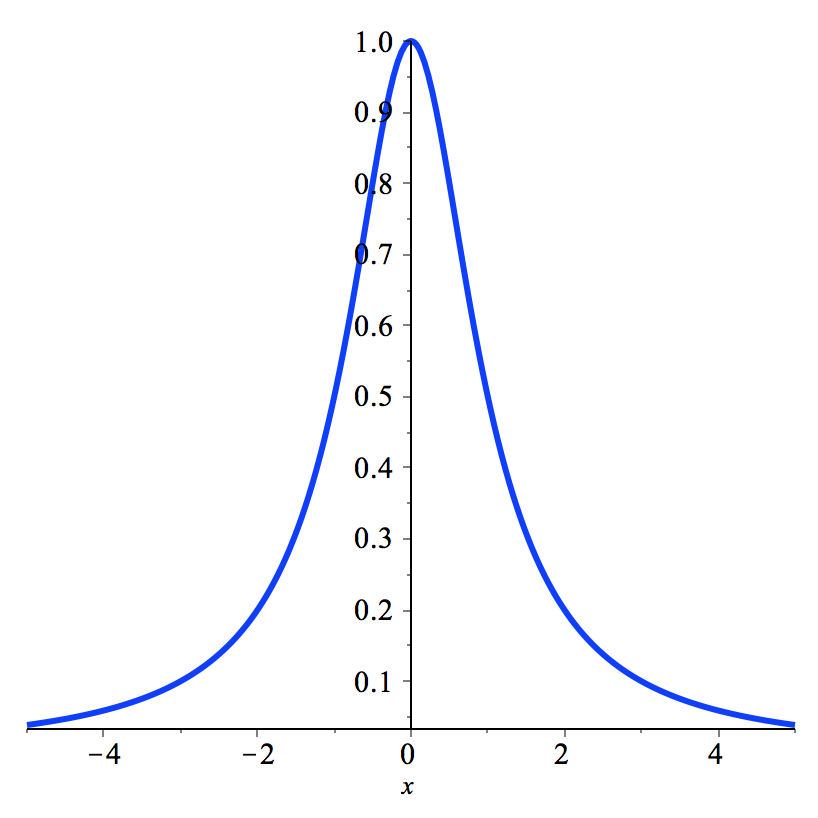
\includegraphics[width=0.9\linewidth, height=4cm]{fig/f7}
    \caption*{$f_7(x)=\frac{1}{1+x^2}$}
    \end{subfigure}
\end{figure}

\subsection*{Solution (ii)}

Using \textbf{definition 5.1.1} the support of a function is defined as: 

\begin{gather*}
    supp\:f=\overline{\{x \in \mathbb{R} | f(x) \neq 0 \}}
\end{gather*}

For $f_6(x)$ the characteristic function forces the function to be zero outside the range of $[-2\pi,2\pi]$ which means, that it automatically has compact support being this interval. Sinus has three incidents where it is zero in this interval, but as the support is the smallest closed set then $-\pi$, 0 and $\pi$ is within the support.
 
\begin{gather*}
    supp\:f_6(x) = \overline{\{x \in \mathbb{R} | f_6(x) \neq 0 \}}=[-2 \pi,2 \pi]
\end{gather*}

For $f_7(x)$ the function never gets to zero, meaning that

\begin{gather*}
    supp\:f_7(x) = \overline{\{x \in \mathbb{R} | f_7(x) \neq 0 \}}=\mathbb{R}
\end{gather*}

So $f_7(x)$ does not have compact support. 
\subsection*{Solution (iii)}

Since $f_6(x)$ is continuous and zero outside $[-2\pi,2\pi]$, $f_6(x) \in C_0(x)$. $f_7(x)$ goes towards zero when $|x| \rightarrow \infty$ while being continuous so $f_7(x) \in C_0(x)$.

\subsection*{Solution (iv)}

Since $f_6(x)$ has compact support and is in $C_0(x)$, $f_6(x)\in C_c(x)$.

\subsection*{Solution (v)}

It is clear to see, that $f_6(x)$ is within $L^1(\mathbb{R})$ being an odd function confined in a finite range by the characteristic function. But for $f_7(x)$ it is not as obvious. 

\begin{gather*}
    \int_{-\infty}^{\infty} \frac{1}{1+x^2} \text{d}x=2  \int_{0}^{\infty} \frac{1}{1+x^2} \text{d}x = \\ 2 \left[ \text{arctan}(x) \right]_0^{\infty}=2 \frac{1}{2}\pi = \pi
\end{gather*}
Which is less than infinity letting it also be in $L^1(\mathbb{R})$. 

\section*{Problem 5.18}
\begin{figure}[H]
    \centering
    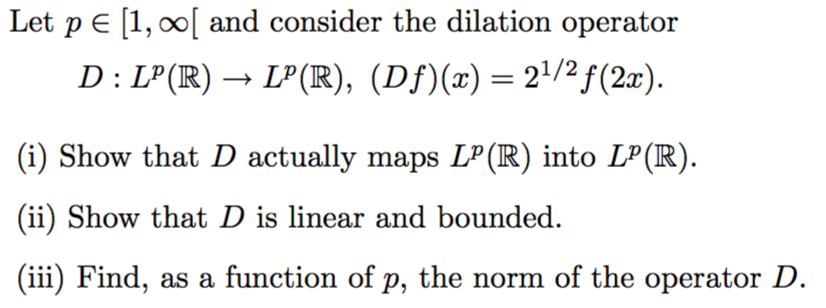
\includegraphics[width=0.8\textwidth]{fig/prob518}
\end{figure}

\subsection*{Solution (i)}

Showing that $D$ is well defined meaning $Df \in L^p(\mathbb{R})$ we might as well look at the norm $||Df||_p < \infty$, giving us

\begin{gather*}
    ||Df||_p = \left( \int_{-\infty}^{\infty}|\sqrt{2}f(2x)|^p \text{d}x\right)^{1/p}=\sqrt{2}\left( \int_{-\infty}^{\infty}|f(2x)|^p \text{d}x\right)^{1/p}
\end{gather*}
Introducing the variable $u=2x$ with $\text{d}x=\frac{1}{2} \text{d}u$:
\begin{gather*}
\sqrt{2}\left( \int_{-\infty}^{\infty}|f(2x)|^p \text{d}x\right)^{1/p}=\sqrt{2}\left( \int_{-\infty}^{\infty}|f(u)|^p \frac{1}{2}\text{d}u\right)^{1/p} = \\
\sqrt{2}\left(\frac{1}{2}\right)^{1/p}\left( \int_{-\infty}^{\infty}|f(u)|^p \text{d}u\right)^{1/p} =\sqrt{2}\left(\frac{1}{2}\right)^{1/p}||f||_p
\end{gather*}
Giving us a finite number times the p norm which is less than infinity, meaning that our operator is well defined.
\subsection*{Solution (ii)}

Linear: Using \textbf{equation (2.6) section 2.4}

\begin{gather*}
    D(\alpha f(x) + \beta g(x))=D((\alpha f + \beta g)(x)) = \sqrt{2}(\alpha f + \beta g)(2x)= \\ 
    \sqrt{2}\alpha f(2x) + \sqrt{2}\beta g(2x) = \alpha D(f(x)) + \beta D(g(x))
\end{gather*}
Meaning the operator is linear. \\

Bounded: Following \textbf{definition 2.4.1} we can use the argumentation from being well defined, and we see that \begin{gather*}
    ||Df||_p \leq K ||f||_p
\end{gather*}
with $K\geq \sqrt{2}\left(\frac{1}{2}\right)^{1/p}$

\subsection*{Solution (iii)}

Again from the argumentation from being well defined, we see that the norm of $D$, the smallest possible value of K, is in fact $||D||=\sqrt{2}\left(\frac{1}{2}\right)^{1/p}$ and therefore a function of $p$. 

\section*{Problem 1.18}
\begin{figure}[H]
    \centering
    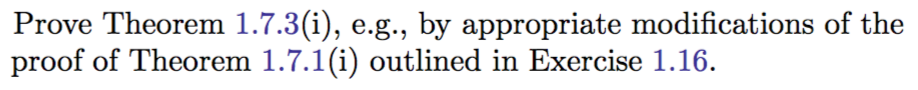
\includegraphics[width=\textwidth]{fig/prob118}
\end{figure}

\subsection*{Solution}
First off, we need Young's inequality which is found by looking at the function $y(x)=x^{p-1}$ and the sketch

\begin{figure}[H]
    \centering
    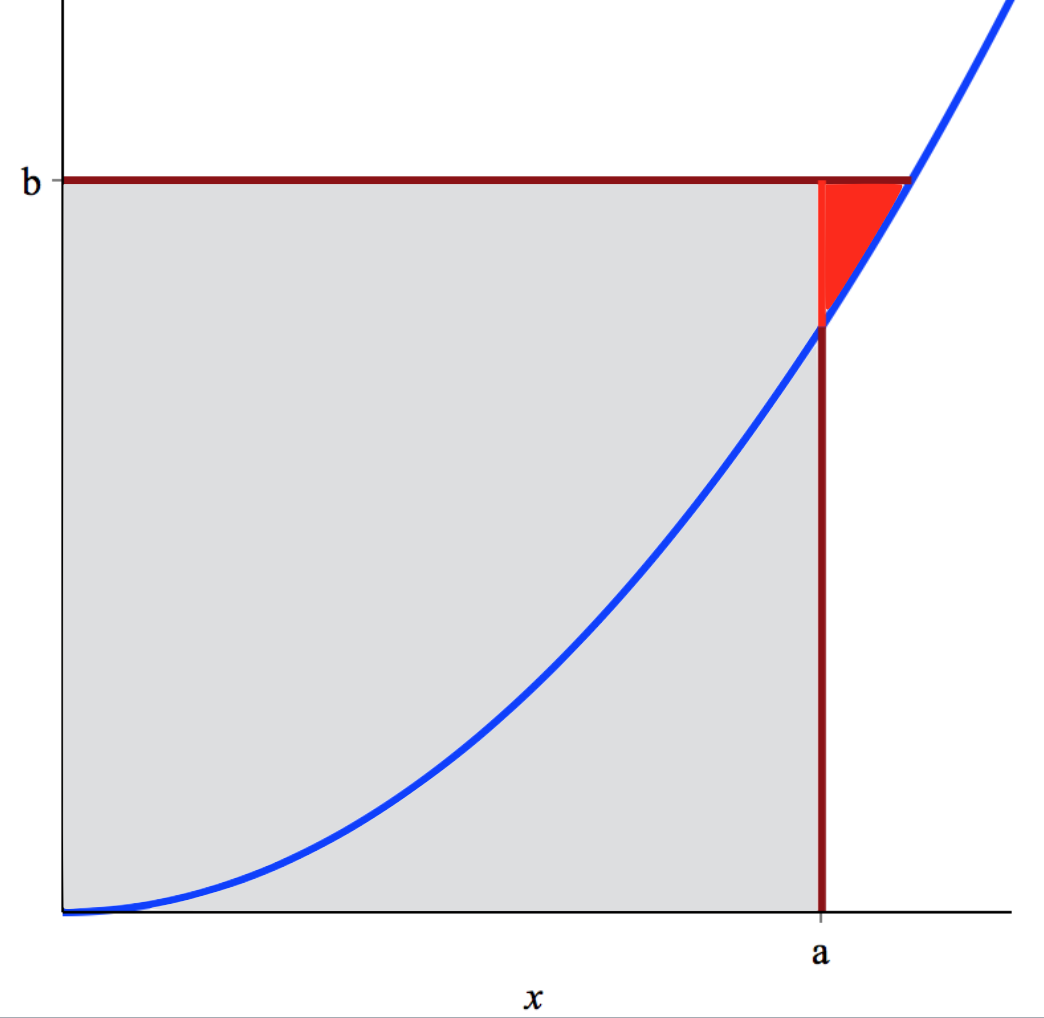
\includegraphics[width=5cm]{fig/sketch}
    \caption*{$y(x)=x^{p-1}$ and the box with sides $ab$}
\end{figure}

Here we see that the area of the box is the smallest value for the sum of the areas under the graph with respect to the x and y axis. This gives us Young's inequality.


\begin{gather*}
\text{Area under the graph with respect to the x-axis} \\
    \int_0^a x^{p-1} \text{d}x = \left[\frac{1}{p}x^p\right]_0^a = \frac{1}{p}a^p
\end{gather*}

\begin{gather*}
\text{Converting to x(y)} \\
    y(x)=x^{p-1} \Rightarrow x(y)=y^{\frac{1}{p-1}}
\end{gather*}
But we know, that 

\begin{gather*}
    \frac{1}{p}+\frac{1}{q}= \frac{p+q}{qp}=1 \Rightarrow p+q = qp \Rightarrow \\
    (q-1)(p-1)=pq-p-q+1 = p+q-p-q+1=1 \Rightarrow \\ 
    q-1 = \frac{1}{p-1}
\end{gather*}
So we can write the function of $x(y)$ as
\begin{gather*}
    x(y)=y^{\frac{1}{p-1}}=y^{q-1}
\end{gather*}

\begin{gather*}
\text{Area under the graph with respect to the y-axis}\\
    \int_0^b y^{q-1} \text{d}y = \left[\frac{1}{q}y^q\right]_0^b = \frac{1}{q}b^q
\end{gather*}
Which ends our inequality as: 
\begin{gather*}
    ab \leq \frac{1}{p}a^p + \frac{1}{q}b^q
\end{gather*}
Now for the actual proof of theorem 1.7.3 (i). If we choose $a$ and $b$ as

\begin{gather*}
    a=\frac{|x_k|}{\left(\sum |x_k|^p\right)^{1/p}} \: \:\text{and}\: \: b= \frac{|y_k|}{\left(\sum |y_k|^q\right)^{1/q}}
\end{gather*}

By using Youngs inequality we get

\begin{gather*}
    ab = \frac{|x_k y_k|}{\left(\sum |x_k|^p\right)^{1/p}\left(\sum |y_k|^q\right)^{1/q}} \leq \frac{1}{p} \frac{|x_k|^p}{\sum |x_k|^p}+\frac{1}{q} \frac{|y_k|^q}{\sum |y_k|^q} \Rightarrow \\
    \sum ab = \frac{\sum|x_k y_k|}{\left(\sum |x_k|^p\right)^{1/p}\left(\sum |y_k|^q\right)^{1/q}} \leq \frac{1}{p} \frac{\sum|x_k|^p}{\sum |x_k|^p}+\frac{1}{q} \frac{\sum|y_k|^q}{\sum |y_k|^q} \Rightarrow \\
    \frac{\sum|x_k y_k|}{\left(\sum |x_k|^p\right)^{1/p}\left(\sum |y_k|^q\right)^{1/q}} \leq \frac{1}{p}+\frac{1}{q}=1 \Rightarrow \\
    \sum|x_k y_k| \leq \left(\sum |x_k|^p\right)^{1/p}\left(\sum |y_k|^q\right)^{1/q} \: \: \square
\end{gather*}
As we wanted.
\end{document}
